\subsection{Fine-tuning fully-connected layers} \label{subsec:fcmodel}

The second approach is to fine-tune only the fully connected layers with the real data. The first convolutional/pooling layers that perform the feature extraction are frozen, which means that during training their weights are not updated. This way we are using a feature extractor trained on synthetic data and with real data we improve only the classification of the network. 

We are using the trained final model from Section \ref{subsec:finalmodel} as a feature extractor, which achieved the accuracy of 81.00 \% on the validation set of real data. Again we are testing various hyperparameters to improve our model. Based on the extensive training we have established a model with following parameters: 

\begin{itemize}
    \setlength\itemsep{1px}
    \item activation function Leaky RELU with a slope of 0.05
    \item batch size of 64
    \item optimizer ADAM with betas = 0.9, 0.999
    \item starting learning rate of $1e^{-3}$
    \item exponential scheduler with $\gamma$ = 0.9
    \item dropout in fully-connected layer with probability of 0.5
    \item L2 regularization with $\lambda$ set to $1e^{-5}$
\end{itemize}

The model achieved an accuracy of 94.33 \% on the real data and 87 \% on the synthetic data on the validation set. While the accuracy on the real data has improved from the model in Section \ref{subsec:finalmodel}, the performance on the synthetic data has decreased significantly. 
The evolution of loss and accuracy during training is illustrated in the Figure \ref{fig:lossaccm33}. 


\begin{figure}[!h]
\centering
    \begin{subfigure}[t]{.45\textwidth}
        \centering
        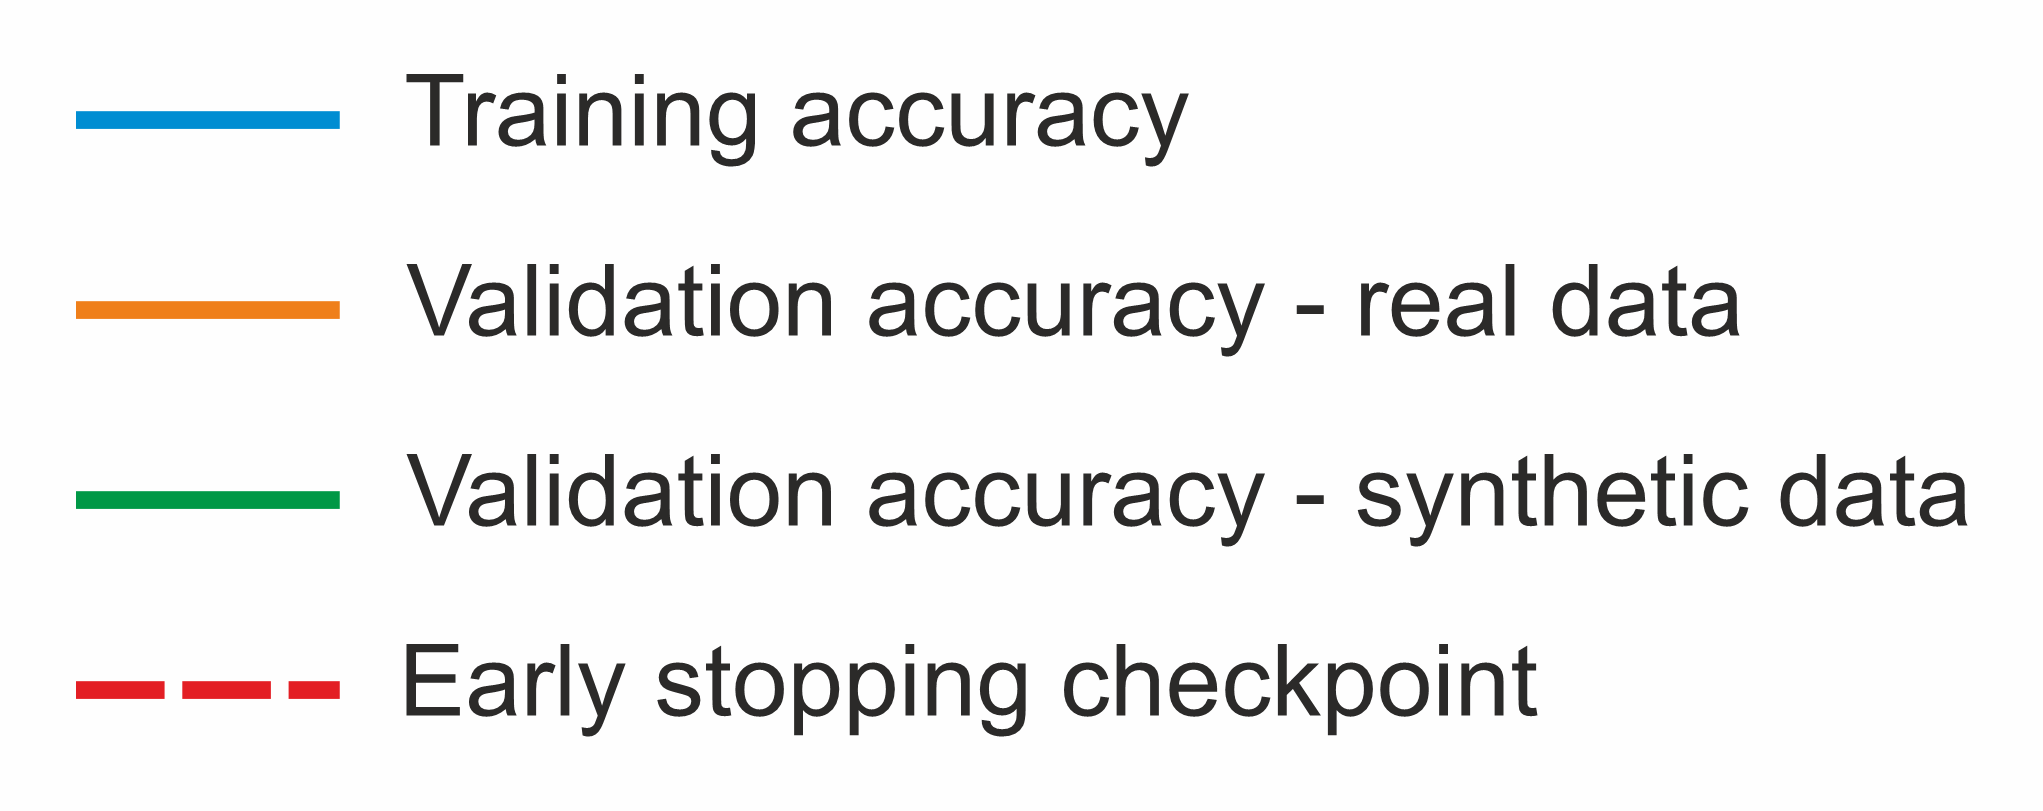
\includegraphics[width=.7\textwidth]{images/popisAc.png}
        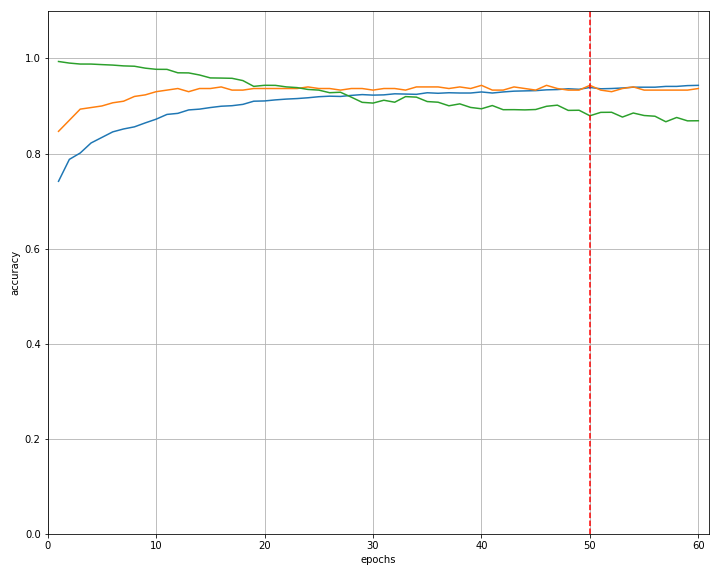
\includegraphics[width=\textwidth]{images/accuracy14fe_0.png}
        \caption{The accuracy during training.}
        \label{fig:accm33}
    \end{subfigure}
    \begin{subfigure}[t]{.45\textwidth}
        \centering
        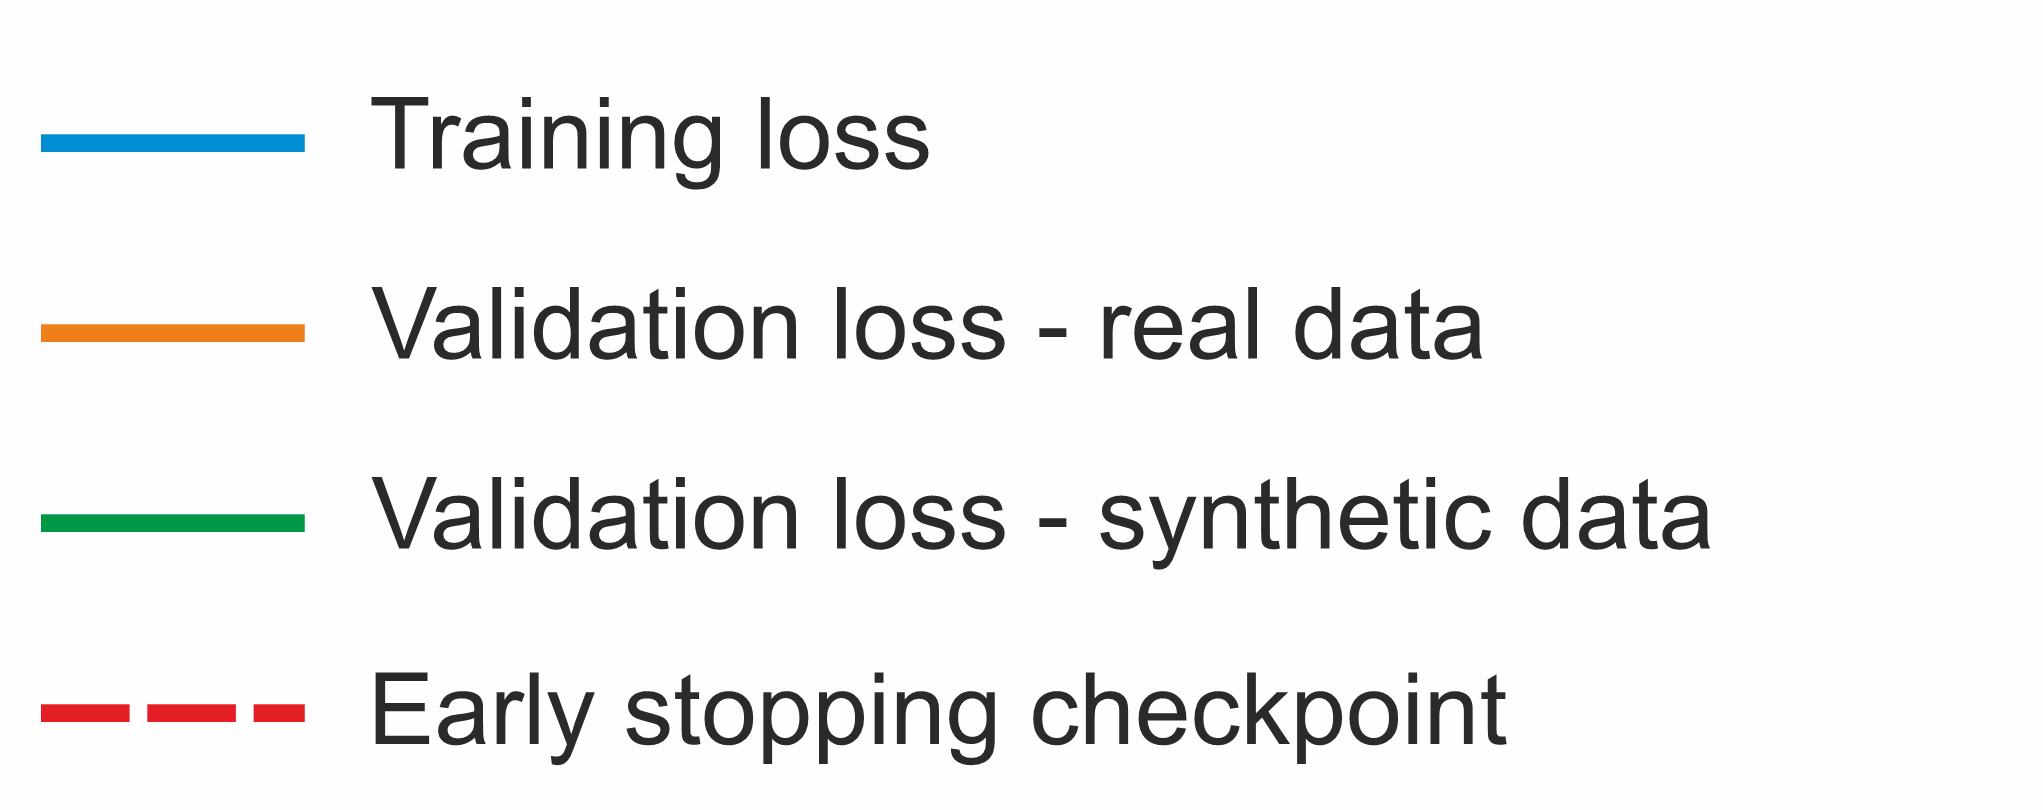
\includegraphics[width=.7\textwidth]{images/popisLoss.png}
        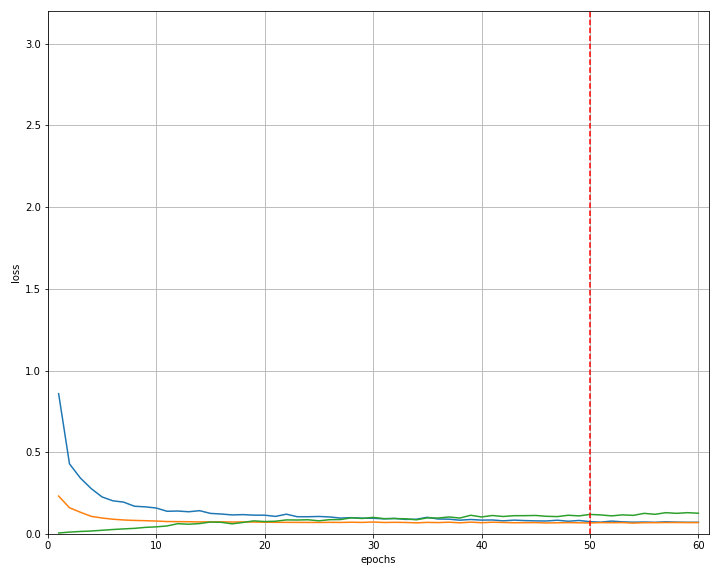
\includegraphics[width=\textwidth]{images/losses14fe_0.png}
        \caption{The loss during training.}
        \label{fig:lossm33}
    \end{subfigure}

    \caption{The evolution of the loss and accuracy during training of the model that has fine-tuned fully-connected layers with real data.}
    \label{fig:lossaccm33}
\end{figure}